\chapter{Ruwe resultaten}%
\label{ch:ruweresultaten}
In dit deel word er over alle ruwe resultaten gegaan. Elke afbeelding in dit hoofdstuk bevatten rechtstreekse resultaten vanuit de XCode Profiler. Bij deze afbeeldingen word er ook een kort woordje uitleg gedaan die de resultaten beschrijven. In dit hoofdstuk word er vaak gesproken over data, de datatype dat hier telkens gebruikt word is een AttributedString.

Voor het meten van het CPU verbruik tijdens het testen van verschillende methoden van data-overdracht is de Xcode profiling tool gebruikt met als template de CPU profiler. Met deze tool is gemeten hoeveel Mc(Mega cycles, cycle = 
de tijd die nodig is voor de uitvoering van één eenvoudige processorbewerking) de app vereist heeft van de CPU per type van data-overdracht. 

Voor het meten van het aantal updates van verschillende view property's, view refreshes en totale CPU gebruik tijd tijdens het testen van verschillende methoden van data-overdracht is de Xcode profiling tool gebruikt met als template de Swift-UI profiler. 

\section{test1: Dataoverdracht in child views}
In deze sectie word de applicatie in de afbeelding hieronder gebruikt om de testen uit te voeren. Opgebouwd uit 1 verticale lijsten die 10 horizontale lijsten bevat per horizontale lijst worden er 10 cellen weergegeven. Elke cel is zeer CPU heavy opgebouwd zodat de resultaten meer zichtbaar worden in de testen. Elke cel bevat ook een knop die een aanpassing van de testbare data gaat triggeren. In volgende afbeelding word de hierarchy afgebeeld. Voor elk type van dataoverdracht is er 10 keer op de button gedrukt voor het wijzigen van de view. Zo zijn de metingen tot stand gekomen. Alle ruwe resultaten die waargenomen zijn per datatype kan u terugvinden in bijlagen onder sectie test1: Dataoverdracht in child views. 
\begin{figure}[H]
    \centering
    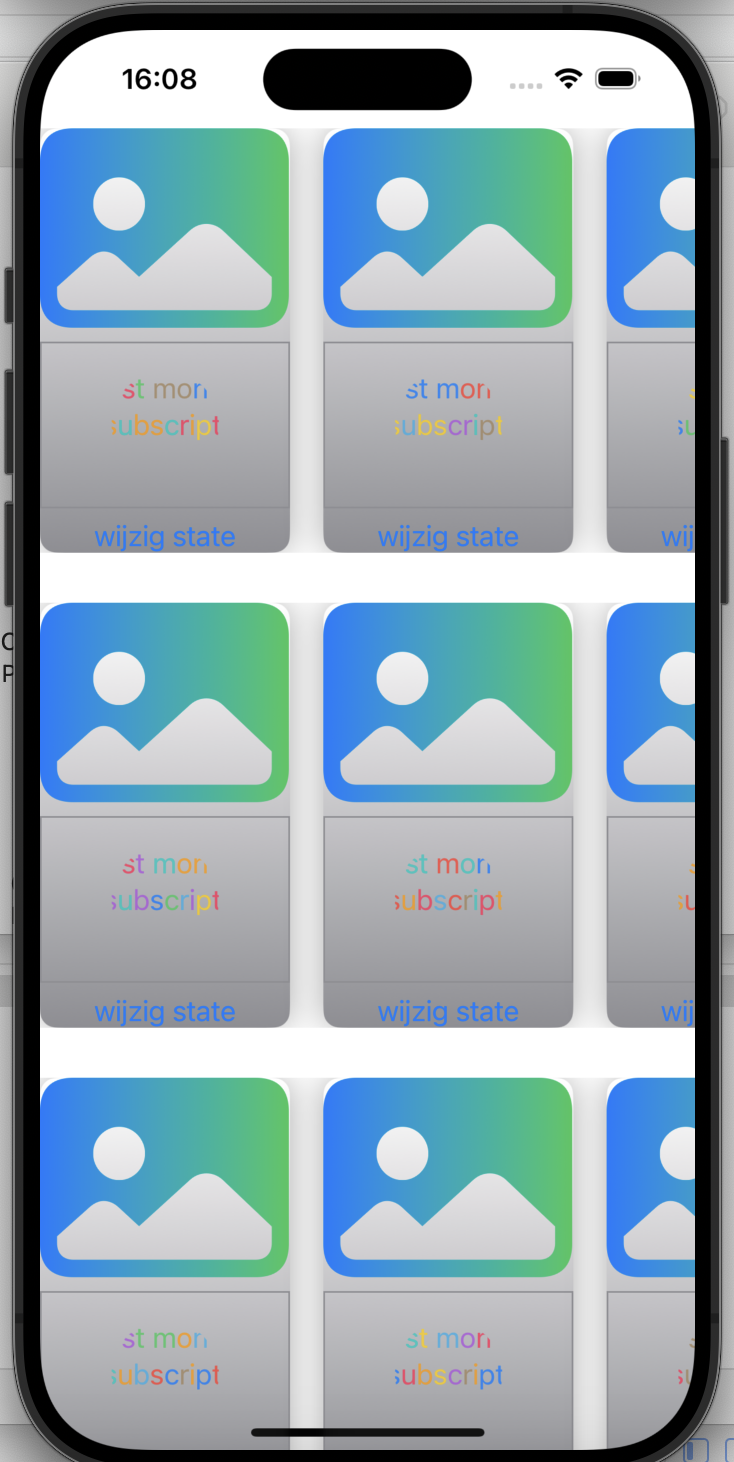
\includegraphics[width=0.4\textwidth]{testapplication} 
    \caption{testapplicatie}
    \label{fig:testapplication}
\end{figure}
\begin{figure}[H]
    \centering
    \includegraphics[width=0.4\textwidth]{bptest1_insubview/dataHierarchy} 
    \caption{testapplicatie data hierarchy}
    \label{fig:testapplicationHierarchy}
\end{figure}

\subsection{Samengevat}
Onderstaande tabel bevat alle samengevatte resultaten uit deze test in 1 tabel gegoten. Uit deze tabel word er later in deze proef een conclusie getrokken.
\newpage
\begin{table}[H]
    \centering
    \begin{tabularx}{\textwidth}{|>{\raggedright\arraybackslash}m{5cm}|X|X|X|X|}
        \hline
        \textbf{Description} & \textbf{Binding} & \textbf{Observable} & \textbf{Environment Object} & \textbf{Observable Object} \\
        \hline
        \multicolumn{5}{|l|}{\textbf{Refresh count}} \\
        \hline
        ContentView refresh count & 0 & 0 & 0 & 0 \\
        \hline
        TileView refresh count & 10 & 10 & 0 & 0 \\
        \hline
        Button refresh count & 10 & 0 & 10 & 10 \\
        \hline
        Total refresh count & 20 & 10 & 10 & 10 \\
        \hline
        \multicolumn{5}{|l|}{\textbf{Refresh duration}} \\
        \hline
        ContentView total refresh duration & N.V.T & N.V.T & N.V.T & N.V.T \\
        \hline
        TileView total refresh duration & 393,62 \textmu s & 1,82 ms & N.V.T & N.V.T \\
        \hline
        Button total refresh duration & 104,46 \textmu s & N.V.T & 214,58 \textmu s & 125,63 \textmu s \\
        \hline
        Total duration & 498,08 \textmu s & 1,82 ms & 214,58 \textmu s & 125,63 \textmu s \\
        \hline
        ContentView average refresh duration & N.V.T & N.V.T & N.V.T & N.V.T \\
        \hline
        TileView average refresh duration & 39,36 \textmu s & 181,93 \textmu s & N.V.T & N.V.T \\
        \hline
        Button average refresh duration & 10,45 \textmu s & N.V.T & 21,56 \textmu s & 12,56 \textmu s \\
        \hline
        \multicolumn{5}{|l|}{\textbf{View property updates}} \\
        \hline
        ContentView property updates & N.V.T & N.V.T & N.V.T & N.V.T \\
        \hline
        TileView property updates & 10 & 10 & 0 & 0 \\
        \hline
        Button property updates & 10 & 0 & 10 & 10 \\
        \hline
        Total property updates & 20 & 10 & 10 & 10 \\
        \hline
        \multicolumn{5}{|l|}{\textbf{CPU usage}} \\
        \hline
        Total CPU usage time & 481 ms & 400 ms & 401 ms & 447 ms \\
        \hline
        Total CPU weight & 245,72 Mc & 294,88 Mc & 243,61 Mc & 653,23 Mc \\
        \hline
    \end{tabularx}
    \caption{Performance metrics comparison}
    \label{tab:performance_metrics}
\end{table}


\section{test2: Dataoverdracht naar meerdere child views met lazyLists}
% Binding test 2
In deze sectie word de applicatie in de afbeelding hieronder gebruikt om de testen uit te voeren. Opgebouwd uit 1 LazyVStack's die 10 LazyHStack's bevat per HStack worden er 10 Tegels weergegeven. Elke tegel is zeer CPU heavy opgebouwd zodat de resultaten meer zichtbaar worden in de testen. Elke tile bevat ook een knop die een aanpassing van de testbare data gaat triggeren. De data word naar elke tile doorgegeven dus heeft invloed op alle child views. In volgende afbeelding word de hierarchy afgebeeld. Voor elk type van dataoverdracht is er 10 keer op de button gedrukt voor het wijzigen van de data die verbonden is met alle view's. Zo zijn de metingen tot stand gekomen. Alle ruwe resultaten die waargenomen zijn per datatype kan u terugvinden in bijlagen onder sectie test2: Dataoverdracht naar meerdere child views met lazyLists.
\begin{figure}[H]
    \centering
    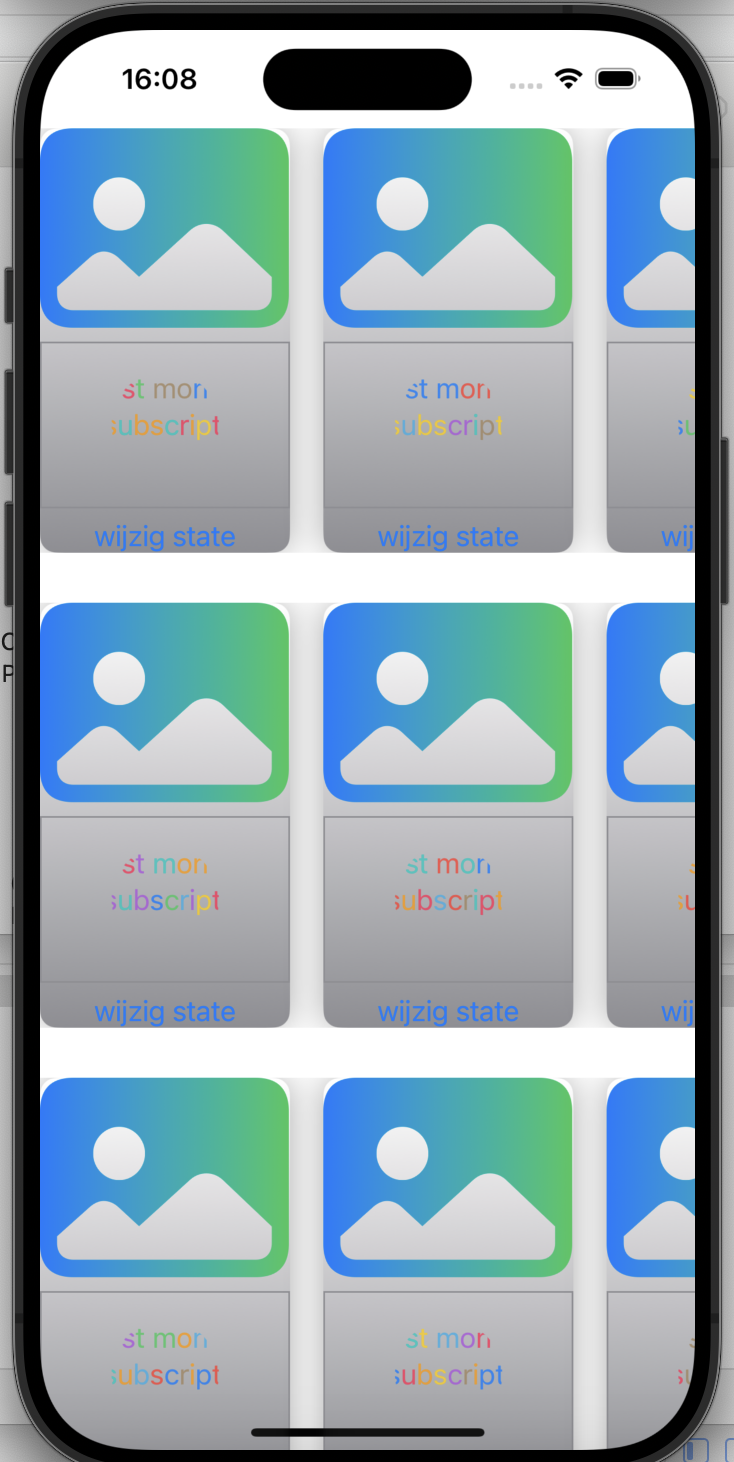
\includegraphics[width=0.4\textwidth]{testapplication} 
    \caption{testapplicatie}
    \label{fig:testapplication2}
\end{figure}
\begin{figure}[H]
    \centering
    \includegraphics[width=0.4\textwidth]{bptest2_lazy/dataHierarchy} 
    \caption{testapplicatie data hierarchy}
    \label{fig:testapplicationHierarchy2}
\end{figure}

\subsection{Samengevat}
Onderstaande tabel bevat alle samengevatte resultaten uit deze test in 1 tabel gegoten. Uit deze tabel word er later in deze proef een conclusie getrokken.
\newpage
\begin{table}[H]
    \centering
    \begin{tabularx}{\textwidth}{|>{\raggedright\arraybackslash}m{5cm}|X|X|X|X|}
        \hline
        \textbf{Description} & \textbf{Binding} & \textbf{Observable} & \textbf{Environment Object} & \textbf{Observable Object} \\
        \hline
        \multicolumn{5}{|l|}{\textbf{Refresh count}} \\
        \hline
        ContentView refresh count & 10 & 1 & 0 & 0 \\
        \hline
        TileView refresh count & 90 & 99 & 90 & 90 \\
        \hline
        Button refresh count & N.V.T & N.V.T & N.V.T & N.V.T \\
        \hline
        Total refresh count & 100 & 100 & 90 & 90 \\
        \hline
        \multicolumn{5}{|l|}{\textbf{Refresh duration}} \\
        \hline
        ContentView total refresh duration & 269,46 \textmu s & 40,25 \textmu s & N.V.T & N.V.T \\
        \hline
        TileView total refresh duration & 1,93 ms & 2,08 ms & 1,85 ms & 2,1 ms \\
        \hline
        Button total refresh duration & N.V.T & N.V.T & N.V.T & N.V.T \\
        \hline
        Total duration & 2,30 ms & 2,12 ms & 1,85 ms & 2,1 ms \\
        \hline
        ContentView average refresh duration & 26,95 \textmu s & 40,25 \textmu s & N.V.T & N.V.T \\
        \hline
        TileView average refresh duration & 21,48 \textmu s & 20,97 \textmu s & 20,50 \textmu s & 23,33 \textmu s \\
        \hline
        Button average refresh duration & N.V.T & N.V.T & N.V.T & N.V.T \\
        \hline
        \multicolumn{5}{|l|}{\textbf{View property updates}} \\
        \hline
        ContentView property updates & 10 & 1 & 0 & 0 \\
        \hline
        TileView property updates & 90 & 9 & 90 & 90 \\
        \hline
        Button property updates & N.V.T & N.V.T & N.V.T & N.V.T \\
        \hline
        Total property updates & 100 & 10 & 90 & 90 \\
        \hline
        \multicolumn{5}{|l|}{\textbf{CPU usage}} \\
        \hline
        Total CPU usage time & 666 ms & 927 ms & 609 ms & 515 ms \\
        \hline
        Total CPU weight & 936,85 Mc & 463,30 Mc & 429,49 Mc & 862,21 Mc \\
        \hline
    \end{tabularx}
    \caption{Performance metrics comparison}
    \label{tab:performance_metrics2}
\end{table}


\section{test3: Dataoverdracht naar meerdere child views}
% Binding test 3
In deze sectie word de applicatie in de afbeelding hieronder gebruikt om de testen uit te voeren. Opgebouwd uit 1 VStack's die 10 HStack's bevat per HStack worden er 10 Tegels weergegeven. Elke tegel is zeer CPU heavy opgebouwd zodat de resultaten meer zichtbaar worden in de testen. Elke tile bevat ook een knop die een aanpassing van de testbare data gaat triggeren. De data word naar elke tile doorgegeven dus heeft invloed op alle child views. In volgende afbeelding word de hierarchy afgebeeld. Voor elk type van dataoverdracht is er 10 keer op de button gedrukt voor het wijzigen van de data die verbonden is met alle view's. Zo zijn de metingen tot stand gekomen. Alle ruwe resultaten die waargenomen zijn per datatype kan u terugvinden in bijlagen onder sectie test3: Dataoverdracht naar meerdere child views.
\begin{figure}[H]
    \centering
    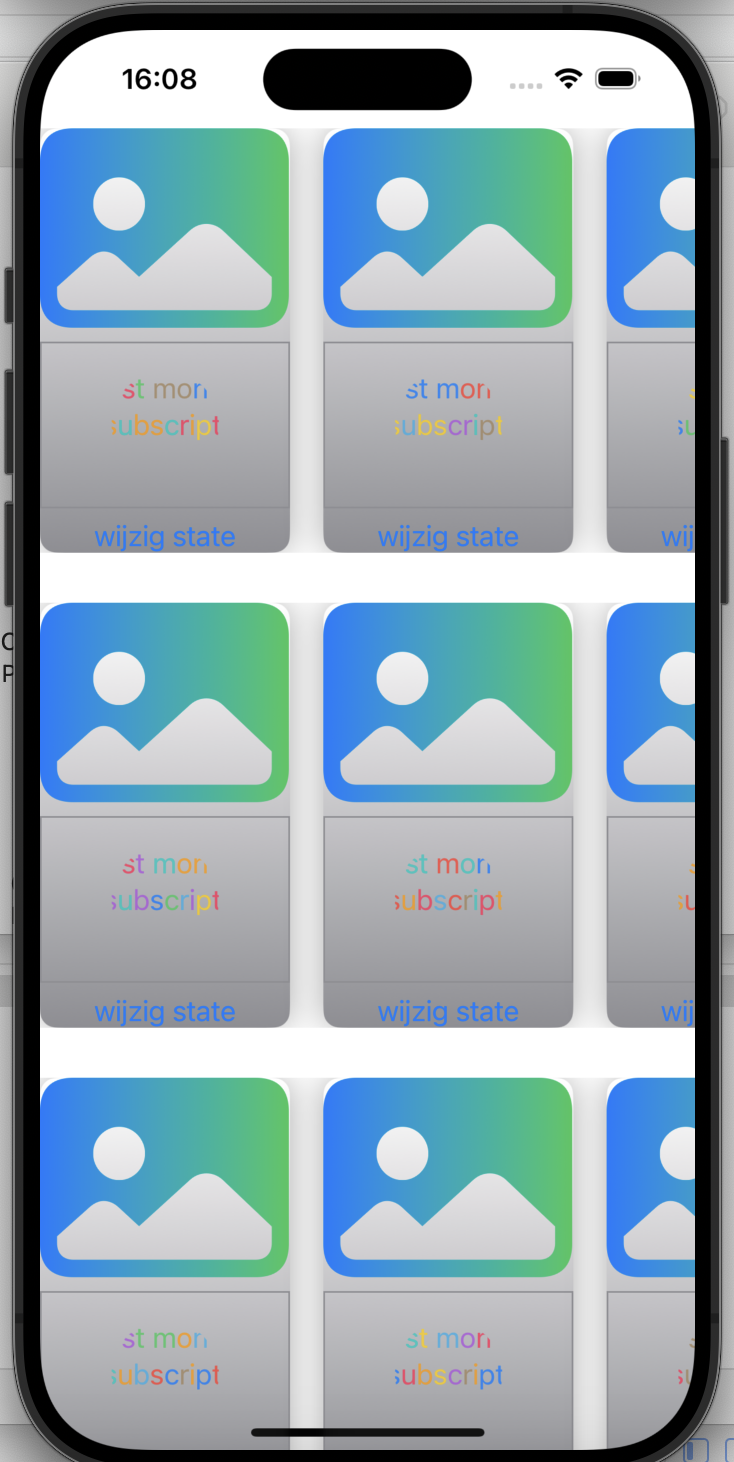
\includegraphics[width=0.4\textwidth]{testapplication} 
    \caption{testapplicatie}
    \label{fig:testapplication3}
\end{figure}
\begin{figure}[H]
    \centering
    \includegraphics[width=0.4\textwidth]{bptest2_lazy/dataHierarchy} 
    \caption{testapplicatie data hierarchy}
    \label{fig:testapplicationHierarchy3}
\end{figure}


\subsection{Samengevat}
Onderstaande tabel bevat alle samengevatte resultaten uit deze test in 1 tabel gegoten. Uit deze tabel word er later in deze proef een conclusie getrokken.
\newpage
\begin{table}[H]
    \centering
    \begin{tabularx}{\textwidth}{|>{\raggedright\arraybackslash}m{5cm}|X|X|X|X|}
        \hline
        \textbf{Description} & \textbf{Binding} & \textbf{Observable} & \textbf{Environment Object} & \textbf{Observable Object} \\ \hline
        \textbf{Refresh count} & & & & \\ \hline
        ContentView refresh count & 10 & 0 & 0 & 0 \\ \hline
        TileView refresh count & 4410 & 4410 & 4410 & 4410 \\ \hline
        Button refresh count & N.V.T & N.V.T & N.V.T & N.V.T \\ \hline
        Total refresh count & 4420 & 4410 & 4410 & 4410 \\ \hline
        \textbf{Refresh duration} & & & & \\ \hline
        ContentView total refresh duration & 209,96 $\mu$s & N.V.T & N.V.T & N.V.T \\ \hline
        TileView total refresh duration & 30,15 ms & 23,24 ms & 24,49 ms & 24,33 ms \\ \hline
        Button total refresh duration & N.V.T & N.V.T & N.V.T & N.V.T \\ \hline
        Total duration & 30,36 ms & 23,24 ms & 24,49 ms & 24,33 ms \\ \hline
        ContentView average refresh duration & 6,87 $\mu$s & N.V.T & N.V.T & N.V.T \\ \hline
        TileView average refresh duration & 6,84 $\mu$s & 5,27 $\mu$s & 5,55 $\mu$s & 5,52 $\mu$s \\ \hline
        Button average refresh duration & N.V.T & N.V.T & N.V.T & N.V.T \\ \hline
        \textbf{View property updates} & & & & \\ \hline
        ContentView property updates & 10 & 0 & 0 & 0 \\ \hline
        TileView property updates & 4410 & 0 & 4410 & 4410 \\ \hline
        Button property updates & N.V.T & N.V.T & N.V.T & N.V.T \\ \hline
        Total property updates & 4420 & 0 & 4410 & 4410 \\ \hline
        \textbf{CPU usage} & & & & \\ \hline
        Total CPU usage time & 6,02 s & 4,8 s & 4,77 s & 4,81 s \\ \hline
        Total CPU weight & 12,93 Gc & 12,19 Gc & 12,10 Gc & 12,04 Gc \\ \hline
    \end{tabularx}
    \caption{Performance metrics}
\end{table}


\chapter{Resultaten}%
\label{ch:resultaten}
In dit hoofdstuk word er dieper in de onderzoeksresultaten van dit onderzoek gedelft. Alle resultaten zijn verkregen door de applicatie te testen via een Iphone 15 pro, IOS 17.4. Alle testen zijn ook systematisch 10 tot 100 keer overlopen voor een correcter resultaat. Van elke test word er nu een vergelijking gemaakt van de verschillende annotaties. Om zo tot een conclusie te komen.

\section{test1: het testen op een lege view met grote dataoverdracht}
Uit deze test blijkt dat de beste methode voor dataoverdracht binnen subviews op alle vlakken, behalve vernieuwingstijd, EnvironmentObject is. Als een snellere vernieuwingstijd vereist is, is ObservableObject een betere keuze, hoewel dit wel resulteert in een verdubbeling van de belasting op de CPU in vergelijking met andere methoden. De slechtste methode in deze test is de nieuwe Observable-macro, waarvan de totale vernieuwingstijd 4 tot 5 keer hoger ligt dan die van de andere methoden. 
\begin{table}[H]
    \centering
    
    \begin{tabularx}{\textwidth}{|>{\raggedright\arraybackslash}m{5cm}|X|X|X|X|}
        \hline
        \textbf{Description} & \textbf{Binding} & \textbf{Observable} & \textbf{Environment Object} & \textbf{Observable Object} \\ 
        \hline
        Total refresh count & \cellcolor{red!50}20 & \cellcolor{green!50}10 & \cellcolor{green!50}10 & \cellcolor{green!50}10 \\ 
        \hline
        Total duration & 214,58 \(\mu\)s & \cellcolor{red!50}1,82 ms & 214,58 \(\mu\)s & \cellcolor{green!50}125,63 \(\mu\)s \\ 
        \hline
        Total property updates & \cellcolor{red!50}20 & \cellcolor{red!50}20 & \cellcolor{green!50}10 & \cellcolor{green!50}10 \\ 
        \hline
        Total CPU usage time & \cellcolor{red!50}481 ms & \cellcolor{green!50}400 ms & \cellcolor{green!50}401 ms & 447 ms \\ 
        \hline
        Total CPU weight & \cellcolor{green!50}245,72 Mc & 294,88 Mc & \cellcolor{green!50}243,61 Mc & \cellcolor{red!50}653,23 Mc \\ 
        \hline
    \end{tabularx}
    \caption{Samengevatte resultaten van test1}
    \label{table:summary1}
\end{table}
\begin{itemize}
    \item \textcolor{green}{\textbf{Groen}}: Beste score
    \item \textcolor{red}{\textbf{Rood}}: Slechtste score
\end{itemize}

\section{test2: Dataoverdracht naar meerdere child views met lazyLists}
Uit deze test blijkt dat de beste methode voor dataoverdracht naar meerdere subview's met lazyLists op alle vlakken, behalve CPU usage time, EnvironmentObject is. Als een snellere CPU usage time vereist is, is ObservableObject een betere keuze, hoewel dit wel resulteert in een verdubbeling van de belasting op de CPU in vergelijking met andere methoden. De relatief slechtste methode in deze test is binding, deze scoort op vrijwel alle aspecten de slechtste score.  
\begin{table}[h!]
    \centering
     \begin{tabularx}{\textwidth}{|>{\raggedright\arraybackslash}m{5cm}|X|X|X|X|}
        \hline
        \textbf{Description} & \textbf{Binding} & \textbf{Observable} & \textbf{Environment Object} & \textbf{Observable Object} \\ 
        \hline
        Total refresh count & \cellcolor{red!50}100 & \cellcolor{red!50}100 & \cellcolor{green!50}90 & \cellcolor{green!50}90 \\ 
        \hline
        ContentView total refresh duration & 269,46 \(\mu\)s & 40,25 \(\mu\)s & N.V.T & N.V.T \\ 
        \hline
        TileView total refresh duration & 1,93 ms & 2,08 ms & 1,85 ms & 2,1 ms \\ 
        \hline
        Total duration & \cellcolor{red!50}2,30 ms & 2,12 ms & \cellcolor{green!50}1,85 ms & 2,1 ms \\ 
        \hline
        ContentView average refresh duration & 26,95 \(\mu\)s & 40,25 \(\mu\)s & N.V.T & N.V.T \\ 
        \hline
        TileView average refresh duration & 21,48 \(\mu\)s & 20,97 \(\mu\)s & 20,50 \(\mu\)s & 23,33 \(\mu\)s \\ 
        \hline
        View property updates & 10 & 1 & 0 & 0 \\ 
        \hline
        TileView property updates & 90 & 9 & 90 & 90 \\ 
        \hline
        Total property updates & \cellcolor{red!50}100 & \cellcolor{green!50}10 & 90 & 90 \\ 
        \hline
        Total CPU usage time & 666 ms & \cellcolor{red!50}927 ms & 609 ms & \cellcolor{green!50}515 ms \\ 
        \hline
        Total CPU weight & \cellcolor{red!50}936,85 Mc & 463,30 Mc & \cellcolor{green!50}429,49 Mc & 862,21 Mc \\ 
        \hline
    \end{tabularx}
    \caption{Samengevatte resultaten van test2}
    \label{table:summary2}
\end{table}

\begin{itemize}
    \item \textcolor{green}{\textbf{Groen}}: Beste score
    \item \textcolor{red}{\textbf{Rood}}: Slechtste score
\end{itemize}
\section{test3: Dataoverdracht naar meerdere child views}
Uit deze test blijkt dat de beste methode voor dataoverdracht naar meerdere subview's op alle vlakken, de nieuwe Observable macro is. EnvironmentObject, ObservableObject scoren bijna even goed als de observable macro. Binding daarintegen scoort op alle criteria het slechtste.
\begin{table}[H]
    \centering
    \begin{tabularx}{\textwidth}{|>{\raggedright\arraybackslash}m{5cm}|X|X|X|X|}
        \hline
        \textbf{Description} & \textbf{Binding} & \textbf{Observable} & \textbf{Environment Object} & \textbf{Observable Object} \\
        \hline
         ContentView refresh count & 10 & 0 & 0 & 0 \\
        \hline
         TileView refresh count & 4410 & 4410 & 4410 & 4410 \\
        \hline
        Total refresh count & \cellcolor{red!50} 4420 & \cellcolor{green!50}4410 & \cellcolor{green!50}4410 & \cellcolor{green!50}4410 \\
        \hline
         ContentView total refresh duration & 209.96 μs & N.V.T & N.V.T & N.V.T \\
        \hline
        TileView total refresh duration & 30.15 ms & 23.24 ms & 24.49 ms & 24.33 ms \\
        \hline
        Total duration &  \cellcolor{red!50}30.36 ms & \cellcolor{green!50}23.24 ms & \cellcolor{green!50}24.49 ms & \cellcolor{green!50}24.33 ms \\
        \hline
        ContentView average refresh duration & 6.87 μs & N.V.T & N.V.T & N.V.T \\
        \hline
        TileView average refresh duration & 6.84 μs & 5.27 μs & 5.55 μs & 5.52 μs \\
        \hline
         ContentView property updates & 10 & 0 & 0 & 0 \\
        \hline
        TileView property updates & 4410 & 0 & 4410 & 4410 \\
        \hline
        Total property updates & \cellcolor{red!50} 4420 & \cellcolor{green!50}0 & 4410 & 4410 \\
        \hline
        Total CPU usage time & \cellcolor{red!50} 6.02 s & \cellcolor{green!50}4.8 s & \cellcolor{green!50}4.77 s & \cellcolor{green!50}4.81 s \\
        \hline
        Total CPU weight & \cellcolor{red!50} 12.93 Gc & \cellcolor{green!50}12.19 Gc & \cellcolor{green!50}12.10 Gc & \cellcolor{green!50}12.04 Gc \\
        \hline
    \end{tabularx}
    \caption{Samengevatte resultaten van test3}
    \label{table:summary3}
\end{table}